\subsubsection{Echo Request or Echo Reply Message (ICMPv4)} 
Nel protocollo \textbf{ICMPv4} la tipologia di messaggio \textit{Echo}, viene usata per ricevere indietro una risposta da un host. 
\vspace{1ex} \newline 
I dati ricevuti nel messaggio di Echo, devono essere restituiti nel messaggio di risposta. 
Inoltre i'identificatore e il numero di sequenza possono essere utilizzati dal 
mittente per facilitare l'abbinamento delle risposte con le richieste.
%Ad esempio, l'identificatore potrebbe essere utilizzato come una porta in TCP o UDP per identificare una 
%sessione e il numero di sequenza potrebbe essere incrementato a ogni richiesta di eco inviata.
Chi risponde alla richiesta Echo, restituisce gli stessi valori nella risposta. 
\vspace{2ex} \newline 
Per creare un messaggio di risposta, gli indirizzi di origine e di destinazione vengono semplicemente invertiti,
il codice da 8 viene modificato in 0 e il checksum viene ricalcolato. 

\subsubsection*{Struttura del pacchetto} 
\begin{bytefield}[bitwidth=1.1em]{32} 
    %\bitbox{8}{0} & \bitbox{8}{1} & \bitbox{8}{2} & \bitbox{8}{3} \\
    \bitheader{0-31} \\
    \bitbox{8}{Type (1B)} & \bitbox{8}{Code (1B)} & \bitbox{16}{Checksum (2B)} \\
    \bitbox{16}{Identifier (2B)} && \bitbox{16}{Sequence Number (2B)} \\
    \bitbox{32}{Data ... ($\geq$ 0B)} 
\end{bytefield}
I campi sono i seguenti: 
\begin{itemize}
    \item Type: 8 per i messaggi Echo Request; 0 per i messaggi Echo Reply.
    \item Code: 0 
    \item Checksum: è il complemento a 16 bit del complemento a uno relativo alla somma del messaggio ICMP 
    (che inizia con il campo Type). Verrà calcolato se il campo è zero. 
    \item Identifier: se il codice = 0; l'identificatore serve per facilitare la corrispondenza tra le richieste Echo e le Risposte Echo. Può essere zero. 
    \item Sequence Number: se il codice = 0; il numero di sequenza serve per facilitare la corrispondenza tra le richieste Echo e le Risposte Echo. Può essere zero. 
\end{itemize}
\vspace{1ex} 
Si sfrutteranno quindi i campi nel seguente modo: 
\begin{itemize}
    \item Il campo \textbf{checksum} non è utilizzabile. 
    Essendo il complemento ad 1 del contenuto del pacchetto, se non combaciasse il pacchetto verrebbe scartato. 
    \item Il campo \textbf{identifier} che siccome serve a definire un identificativo delle richieste, può essere un qualsiasi valore. 
    \item Il campo di \textbf{sequenza} potrebbe essere utilizzato per inserire le informazioni; 
    tuttavia, dalle specifiche \href{https://www.rfc-editor.org/rfc/rfc792.html#:~:text=Echo%20or%20Echo%20Reply%20Message}{RFC 792}, esso viene incrementato ad ogni richiesta inviata. 
    Quindi se il valore del campo è troppo variabile, potrebbe risultare sospetto. 
\end{itemize}

\subsubsection*{Analisi complessiva} 
Per l'analisi supponiamo di mandare due comandi che sono: 
\begin{itemize}
    \item \textbf{echo 'Ciao'}: che sono \textit{11 byte} (e quindi \textit{88 bit}\footnote{\label{note:echo:analisi}Ciò sarà utile per i \textit{Timing Covert Channel}})
    \item \textbf{cd /home/marco; ls -l}: che sono \textit{21 byte}  (e quindi \textit{168 bit}\textsuperscript{\ref{note:echo:analisi}}) %\footnotemark[2]
\end{itemize}
Sappiamo che nel caso migliore la capacità di trasmissione di ogni pacchetto è \textbf{2 byte} \label{echo:casoA}; 
questo perchè il campo \textit{identifier} ha una lunghezza di soli \textit{2 byte}. %20
\begin{itemize}
    \item Ogni pacchetto del caso (che chiameremo \hyperref[echo:casoA]{A}) trasporterà \textbf{8 byte}
    \footnote{8 per i campi ICMP presenti}
    (supponendo che non si inseriscano dati) 
\end{itemize} 
Ora si analizza quanti pacchetti saranno necessari per inviare i comandi. \newline
Nel caso si mandasse il comando \textbf{echo 'Ciao'} il numero di pacchetti necessari sarebbere: 
\begin{itemize}
    \item Caso \hyperref[echo:casoA]{A}: Sarebbero necessari \textit{6 pacchetti}. 
    E quindi siccome ogni pacchetto trasporta \textit{8 byte}; si spediranno in totale \textbf{48 byte}. 
\end{itemize} 
Ora analiziamo il comando \textbf{cd /home/marco; ls -l} e quanti pacchetti saranno necessari: 
\begin{itemize}
    \item Caso \hyperref[echo:casoA]{A}: siccome è di \textit{21 byte}, servirebbero \textit{11 pacchetti}. 
    Quindi siccome ogni pacchetto trasporta \textit{8 byte}; si spediranno in totale \textbf{88 byte}. 
\end{itemize}

\begin{center} 
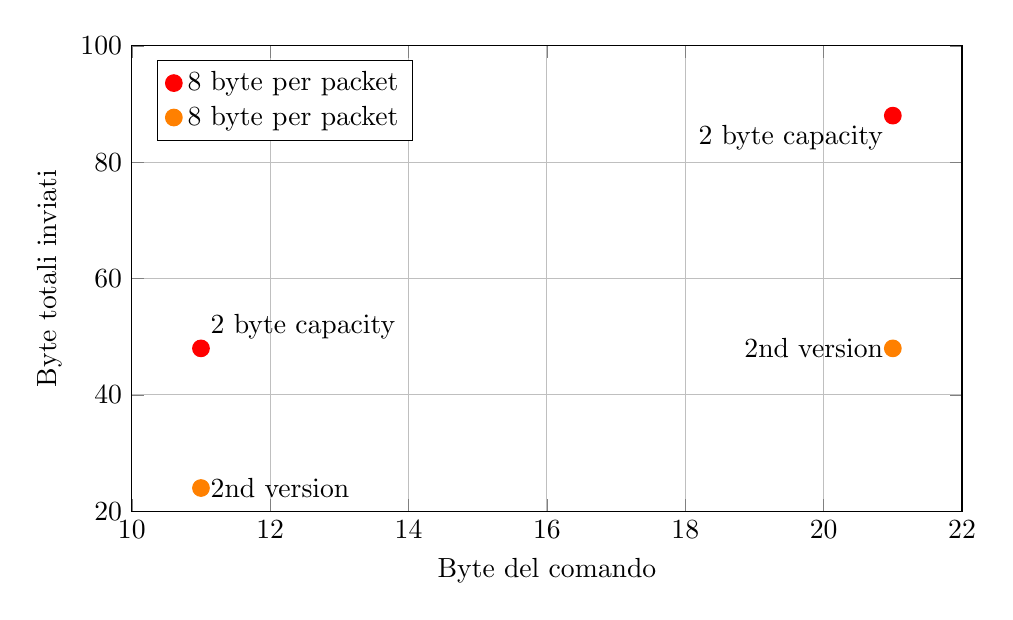
\begin{tikzpicture} 
    \tikzset{
    cmd11/.style={circle,fill=red,inner sep=2pt},
    cmd21/.style={circle,fill=blue,inner sep=2pt}
}
\begin{axis}[
    xlabel={Byte del comando}, 
    ylabel={Byte totali inviati},
    grid=major,
    width=\textwidth,
    height=0.618\textwidth, 
    domain=10:22,
    ymin=20,
    ymax=100, 
    legend pos=north west,
    legend entries={8 byte per packet, 8 byte per packet}
]  
% Plot points
\addplot[only marks, mark=*, mark size=3pt, red] 
coordinates {(11,48) (21,88)}; 
\addplot[only marks, mark=*, mark size=3pt, orange] 
coordinates {(11,24) (21,48)}; 
% Add labels for the points 
\node[above right] at (axis cs:11,48) {2 byte capacity}; 
\node[below left] at (axis cs:21,88) {2 byte capacity}; 

\node[right] at (axis cs:11,24) {2nd version}; 
\node[left] at (axis cs:21,48) {2nd version}; 

\end{axis}
\end{tikzpicture}
\caption{Analisi tempi esecuzione \textit{Echo}} 
\label{table:echo:bytetotali:bytecomando}
\end{center}
Dall'analisi segue che il metodo \hyperref[echo:casoA]{A} non riuslta il migliore. 
Infatti analizzando il caso in cui si usasse anche il campo di \textit{sequenza} [Tabella:\ref{table:echo:bytetotali:bytecomando} Arancione]; 
si avrà una notevole differenza di bytes spediti totalmente rispetto al caso \hyperref[echo:casoA]{A}. 
Tuttavia siccome l'uso di questo campo comporta una maggiore visibilità, 
si sceglie di non usarlo e correre il rischio. Questo comporterà l'invio di un maggior numero di bytes; 
che anche ciò potrebbe rivelare il Covert Channel. 
\vspace{1ex} \newline 
Si è scelto quindi di usare il metodo \hyperref[echo:casoA]{A} ed affidarsi ai meccanismi di difesa presenti nella vittima; 
nella speranza che un numero elevato di pacchetti, ma senza il campo \textit{dati}, possano essere considerati innocqui.
\vspace{2ex} \newline 
Un \textbf{metodo maggiormente efficace} è proprio l'uso del campo \textbf{data}. 
Tuttavia anche questo approccio potrebbe destare sospetti. 
Infatti si dovrà decidere se mandare i dati in chiaro o cifrati:
\begin{itemize}
    \item Nel primo caso sarà possibile leggerne il contenuto. 
    \item Nell'altro, invece, la non possibilità di leggerne il ocntenuto rende lo scambio sospetto. 
    Siccome esistono canali migliori per poter scambiare informazioni in questo modo. 
\end{itemize} 
Inoltre bisognerebbe calcolare la capacità minima afifnche questo campo non risulti anomalo, ma sicuramente sarà maggiore di 2 byte. 
Questo lo si può affermare dopo aver testato i programmi di ping sia su Linux che su Windows. 

\subsubsection{Echo Request or Echo Reply Message (ICMPv6)} 
Nel protocollo \textbf{ICMPv6} la tipologia di messaggio \textit{Echo}, viene usata per ricevere indietro una risposta da un host. 
In questi casi, una \textit{Echo Reply} dovrebbe essere inviata in risposta alla messaggio di \textit{Echo Request}. 
E non vi è alcuna limitazione alla quantità di dati inseribili nei messaggi \textit{Echo}. 
\vspace{1ex} \newline 
I dati ricevuti dall \textit{Echo Request}, dovranno essere restituiti nel messaggio di risposta integralmente e senza modifiche. 
Inoltre i'identificatore e il numero di sequenza possono essere utilizzati dal 
mittente per facilitare l'abbinamento delle risposte con le richieste.
%Ad esempio, l'identificatore potrebbe essere utilizzato come una porta in TCP o UDP per identificare una 
%sessione e il numero di sequenza potrebbe essere incrementato a ogni richiesta di eco inviata.
Inoltre nel messaggio di \textit{Echo Reply}, l'indirizzo sorgente deve essere lo stesso dell'indirizzo di destinazione presente nel messaggio di \textit{Echo Request}.
\vspace{1ex} \newline 
Per creare un messaggio di risposta, gli indirizzi di origine e di destinazione vengono semplicemente invertiti,
il codice da 128 viene modificato in 129 e il checksum viene ricalcolato. 
In aggiunta, ogni nodo deve implementare una funzione di risposta ai messaggi \textit{Echo ICMPv6} così che 
quando riceve delle richieste Echo, generi le relative risposte. 
\vspace{2ex} \newline
%A node SHOULD also implement an application-layer interface for originating Echo Requests and receiving Echo Replies, for diagnostic purposes.
%E inoltre, un nodo dovrebbe implementare un'interfaccia a livello applicazione per poter generare Richieste Echo e ricevere Risposte Echo, a fini diagnostici.
I messaggi \textit{Echo Request} possono essere passati ai processi che ricevono i messaggi \textit{ICMP}. 
Identica cosa i messaggi di \textit{Echo Reply}. 
Essi devono essere trasmessi al processo che ha originato il messaggio di richiesta. 
Inoltre un messaggio di risposta, può essere trasmesso a processi che non hanno originato il messaggio \textit{Echo Request}. 

\subsubsection*{Struttura del pacchetto} 
\begin{bytefield}[bitwidth=1.1em]{32} 
    %\bitbox{8}{0} & \bitbox{8}{1} & \bitbox{8}{2} & \bitbox{8}{3} \\
    \bitheader{0-31} \\
    \bitbox{8}{Type (1B)} & \bitbox{8}{Code (1B)} & \bitbox{16}{Checksum (2B)} \\
    \bitbox{16}{Identifier (2B)} && \bitbox{16}{Sequence Number (2B)} \\
    \bitbox{32}{Data ... ($\geq$ 0B)} 
\end{bytefield}
I campi sono i seguenti: 
\begin{itemize} 
    \item Type: 128 per i messaggi Echo Request; 129 per i messaggi Echo Reply.
    \item Code: 0 
    \item Checksum: è il complemento a 16 bit del complemento a uno relativo alla somma del messaggio ICMP 
    (che inizia con il campo Type). Verrà calcolato se il campo è zero. 
    \item Identifier: se il codice = 0; l'identificatore serve per facilitare la corrispondenza tra le richieste Echo e le Risposte Echo. Può essere zero. 
    \item Sequence Number: se il codice = 0; il numero di sequenza serve per facilitare la corrispondenza tra le richieste Echo e le Risposte Echo. Può essere zero. 
\end{itemize}
\vspace{1ex} 
Si sfrutteranno quindi i campi nel seguente modo: 
\begin{itemize}
    \item Il campo \textbf{checksum} non è utilizzabile. 
    Essendo il complemento ad 1 del contenuto del pacchetto, se non combaciasse il pacchetto verrebbe scartato. 
    \item Il campo \textbf{identifier} che siccome serve a definire un identificativo delle richieste, può essere un qualsiasi valore. 
    \item Il campo di \textbf{sequenza} potrebbe essere utilizzato per inserire le informazioni; 
    tuttavia, dalle specifiche \href{https://www.rfc-editor.org/rfc/rfc4443#section-4.1}{RFC 4443}, esso viene incrementato ad ogni richiesta inviata. 
    Quindi se il valore del campo è troppo variabile, potrebbe risultare sospetto. 
\end{itemize}

\subsubsection*{Analisi complessiva} 
Per l'analisi supponiamo di mandare due comandi che sono: 
\begin{itemize}
    \item \textbf{echo 'Ciao'}: che sono \textit{11 byte} (e quindi \textit{88 bit}\footnote{\label{note:echo6:analisi}Ciò sarà utile per i \textit{Timing Covert Channel}})
    \item \textbf{cd /home/marco; ls -l}: che sono \textit{21 byte}  (e quindi \textit{168 bit}\textsuperscript{\ref{note:echo6:analisi}}) %\footnotemark[2]
\end{itemize}
Sappiamo che nel caso migliore la capacità di trasmissione di ogni pacchetto è \textbf{2 byte} \label{echo6:casoA}; 
questo perchè il campo \textit{identifier} ha una lunghezza di soli \textit{2 byte}. %20
\begin{itemize}
    \item Ogni pacchetto del caso (che chiameremo \hyperref[echo6:casoA]{A}) trasporterà \textbf{8 byte}
    \footnote{8 per i campi ICMP}
    (supponendo che non si inseriscano dati) 
\end{itemize} 
Ora si analizza quanti pacchetti saranno necessari per inviare i comandi. \newline
Nel caso si mandasse il comando \textbf{echo 'Ciao'} il numero di pacchetti necessari sarebbere: 
\begin{itemize}
    \item Caso \hyperref[echo6:casoA]{A}: Sarebbero necessari \textit{6 pacchetti}. 
    E quindi siccome ogni pacchetto trasporta \textit{8 byte}; si spediranno in totale \textbf{48 byte}. 
\end{itemize} 
Ora analiziamo il comando \textbf{cd /home/marco; ls -l} e quanti pacchetti saranno necessari: 
\begin{itemize}
    \item Caso \hyperref[echo6:casoA]{A}: siccome è di \textit{21 byte}, servirebbero \textit{11 pacchetti}. 
    Quindi siccome ogni pacchetto trasporta \textit{8 byte}; si spediranno in totale \textbf{88 byte}. 
\end{itemize}

\begin{center} 
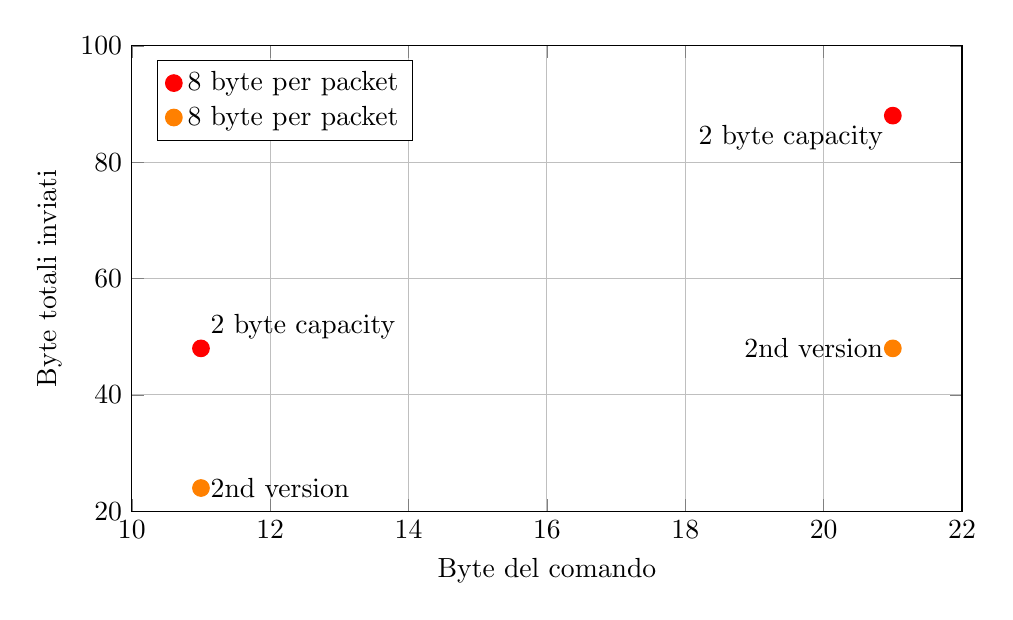
\begin{tikzpicture} 
    \tikzset{
    cmd11/.style={circle,fill=red,inner sep=2pt},
    cmd21/.style={circle,fill=blue,inner sep=2pt}
}
\begin{axis}[
    xlabel={Byte del comando}, 
    ylabel={Byte totali inviati},
    grid=major,
    width=\textwidth,
    height=0.618\textwidth, 
    domain=10:22,
    ymin=20,
    ymax=100, 
    legend pos=north west,
    legend entries={8 byte per packet, 8 byte per packet}
]  
% Plot points
\addplot[only marks, mark=*, mark size=3pt, red] 
coordinates {(11,48) (21,88)}; 
\addplot[only marks, mark=*, mark size=3pt, orange] 
coordinates {(11,24) (21,48)}; 
% Add labels for the points 
\node[above right] at (axis cs:11,48) {2 byte capacity}; 
\node[below left] at (axis cs:21,88) {2 byte capacity}; 

\node[right] at (axis cs:11,24) {2nd version}; 
\node[left] at (axis cs:21,48) {2nd version}; 

\end{axis}
\end{tikzpicture}
\caption{Analisi tempi esecuzione \textit{Echo}} 
\label{table:echo6:bytetotali:bytecomando}
\end{center}
Dall'analisi segue che il metodo \hyperref[echo6:casoA]{A} non riuslta il migliore. 
Infatti analizzando il caso in cui si usasse anche il campo di \textit{sequenza} [Tabella:\ref{table:echo6:bytetotali:bytecomando} Arancione]; 
si avrà una notevole differenza di bytes spediti totalmente rispetto al caso \hyperref[echo6:casoA]{A}. 
Tuttavia siccome l'uso di questo campo comporta una maggiore visibilità, 
si sceglie di non usarlo e correre il rischio. Questo comporterà l'invio di un maggior numero di bytes; 
che anche ciò potrebbe rivelare il Covert Channel. 
\vspace{1ex} \newline 
Si è scelto quindi di usare il metodo \hyperref[echo6:casoA]{A} ed affidarsi ai meccanismi di difesa presenti nella vittima; 
nella speranza che un numero elevato di pacchetti, ma senza il campo \textit{dati}, possano essere considerati innocqui.
\vspace{2ex} \newline 
Un \textbf{metodo maggiormente efficace} è proprio l'uso del campo \textbf{data}. 
Tuttavia anche questo approccio potrebbe destare sospetti. 
Infatti si dovrà decidere se mandare i dati in chiaro o cifrati:
\begin{itemize}
    \item Nel primo caso sarà possibile leggerne il contenuto. 
    \item Nell'altro, invece, la non possibilità di leggerne il ocntenuto rende lo scambio sospetto. 
    Siccome esistono canali migliori per poter scambiare informazioni in questo modo. 
\end{itemize} 
Inoltre bisognerebbe calcolare la capacità minima afifnche questo campo non risulti anomalo, ma sicuramente sarà maggiore di 2 byte. 
Questo lo si può affermare dopo aver testato i programmi di ping sia su Linux che su Windows. 



\subsubsection{Timestamp or Timestamp Reply Message (ICMPv4)} 
Nel protocollo \textbf{ICMPv4} la tipologia di messaggio \textit{Timestamp}, viene usata per ricevere indietro una risposta da un host. 
\vspace{1ex} \newline 
L'identificatore e il numero di sequenza possono essere utilizzati dal mittente del pacchetto per facilitare l'abbinamento delle risposte con le richieste.
%Ad esempio, l'identificatore potrebbe essere utilizzato come una porta in TCP o UDP per identificare una sessione e il numero di sequenza potrebbe essere incrementato a ogni richiesta inviata.
%La destinazione restituisce gli stessi valori nella risposta. 
Inoltre i dati ricevuti nel messaggio di richiesta, vengono restituiti in quello di risposta insieme a dei timestamp aggiuntivi. 
Il timestamp è pari a 32 bit e indica i millisecondi che sono passati dalla mezzanotte UT.
%Un utilizzo di questi timestamp è descritto da Mills [5].
\vspace{1ex} \newline 
Se l'ora non è disponibile in millisecondi o non può essere fornita rispetto alla mezzanotte UT, 
è possibile inserire qualsiasi ora in un timestamp, a condizione che anche il bit di ordine superiore del 
timestamp sia impostato per indicare questo valore non standard. 
\vspace{1ex} \newline  
In un messaggio di risposta, l'indirizzo della sorgente sarà la destinazione. 
Quindi per poter creare un messaggio di risposta timestamp, gli indirizzi di sorgente e destinazione vengono semplicemente invertiti, il codice di tipo viene modificato in 14 e il checksum viene ricalcolato.

\subsubsection*{Struttura del pacchetto} 
\begin{bytefield}[bitwidth=1.1em]{32} 
    %\bitbox{8}{0} & \bitbox{8}{1} & \bitbox{8}{2} & \bitbox{8}{3} \\
    \bitheader{0-31} \\
    \bitbox{8}{Type (1B)} & \bitbox{8}{Code (1B)} & \bitbox{16}{Checksum (2B)} \\
    \bitbox{16}{Identifier (2B)} && \bitbox{16}{Sequence Number (2B)} \\ 
    \bitbox{32}{Originate Timestamp (4B)} \\
    \bitbox{32}{Receive Timestamp (4B)} \\
    \bitbox{32}{Transmit Timestamp (4B)} \\
    \bitbox{32}{Data ... ($\geq$ 0B)} 
\end{bytefield}
I campi sono i seguenti: 
\begin{itemize}
    \item Type: 13 per i messaggi Timestamp Request; 14 per i messaggi Timestamp Reply.
    \item Code: 0 può essere ricevuto da un gateway o da un host
    \item Checksum: è il complemento a 16 bit del complemento a uno relativo alla somma del messaggio ICMP 
    (che inizia con il campo Type). Verrà calcolato se il campo è zero. 
    \item Identifier: se il codice = 0; l'identificatore serve per facilitare la corrispondenza tra le richieste Echo e le Risposte Echo. Può essere zero. 
    \item Sequence Number: se il codice = 0; il numero di sequenza serve per facilitare la corrispondenza tra le richieste Echo e le Risposte Echo. Può essere zero. 
    \item Originate Timestamp: tempo in cui il mittente ha toccato il messaggio per l'ultima volta prima di inviarlo. 
    \item Receive Timestamp: tempo in cui il destinatario ha toccato per la prima volta il messaggio (alla ricezione). 
    \item Transmit Timestamp: tempo in cui il destinatario ha toccato il messaggio per l'ultima volta prima di inviarlo. 
\end{itemize}  
Si sfrutteranno quindi i campi nel seguente modo: 
\begin{itemize}
    \item Il campo \textbf{checksum} non è utilizzabile. 
    Essendo il complemento ad 1 del contenuto del pacchetto, se non combaciasse il pacchetto verrebbe scartato. 
    \item Il campo \textbf{identifier} che siccome serve a definire un identificativo delle richieste, può essere un qualsiasi valore. 
    \item Il campo di \textbf{sequenza} potrebbe essere utilizzato per inserire le informazioni; 
    tuttavia, dalle specifiche \href{https://www.rfc-editor.org/rfc/rfc792.html#:~:text=Timestamp%20or%20Timestamp%20Reply%20Message}{RFC 792}, esso viene incrementato ad ogni richiesta inviata. %%20 
    Quindi se il valore del campo è troppo variabile, potrebbe risultare sospetto. 
    \item I campi \textbf{originate timestamp}, \textbf{receive timestamp}, \textbf{transmit timestamp} dovranno contenere solo il tempo in milliseocndi dalla mezzanotte UT. 
    Quindi in ognuno dei campi può essere inserito un byte nella parte indicante i millisecondi. 
    Si potrebbero inserire un numero magigore di dati sfruttando l'intera lunghezza dei campi ma poi i tempi non risulterebbero congruenti fra di loro
    \footnote{Si potrebbe avere il caso che il destinatario ha modificato il messagio prima di poterlo ricevere}
\end{itemize}

\subsubsection*{Analisi complessiva} 
Per l'analisi supponiamo di mandare due comandi che sono: 
\begin{itemize}
    \item \textbf{echo 'Ciao'}: che sono \textit{11 byte} (e quindi \textit{88 bit}\footnote{\label{note:timestamp:analisi}Ciò sarà utile per i \textit{Timing Covert Channel}})
    \item \textbf{cd /home/marco; ls -l}: che sono \textit{21 byte}  (e quindi \textit{168 bit}\textsuperscript{\ref{note:timestamp:analisi}}) %\footnotemark[2]
\end{itemize}
Sappiamo che nel caso migliore la capacità di trasmissione di ogni pacchetto è \textbf{5 byte} \label{timestamp:casoA}; 
questo perchè il campo \textit{identifier} ha una lunghezza di \textit{2 byte} mentre i tre campi timestamp contengono \textit{un byte} ciascuno. %20
\begin{itemize}
    \item Ogni pacchetto del caso (che chiameremo \hyperref[timestamp:casoA]{A}) trasporterà \textbf{20 byte} 
    \footnote{20 per i campi ICMP} 
\end{itemize} 
Ora si analizza quanti pacchetti saranno necessari per inviare i comandi. \newline
Nel caso si mandasse il comando \textbf{echo 'Ciao'} il numero di pacchetti necessari sarebbere: 
\begin{itemize}
    \item Caso \hyperref[timestamp:casoA]{A}: Sarebbero necessari \textit{3 pacchetti}. 
    E quindi siccome ogni pacchetto trasporta \textit{20 byte}; si spediranno in totale \textbf{60 byte}. 
\end{itemize} 
Ora analiziamo il comando \textbf{cd /home/marco; ls -l} e quanti pacchetti saranno necessari: 
\begin{itemize}
    \item Caso \hyperref[timestamp:casoA]{A}: siccome è di \textit{21 byte}, servirebbero \textit{5 pacchetti}. 
    Quindi siccome ogni pacchetto trasporta \textit{20 byte}; si spediranno in totale \textbf{100 byte}. 
\end{itemize}

\begin{center} 
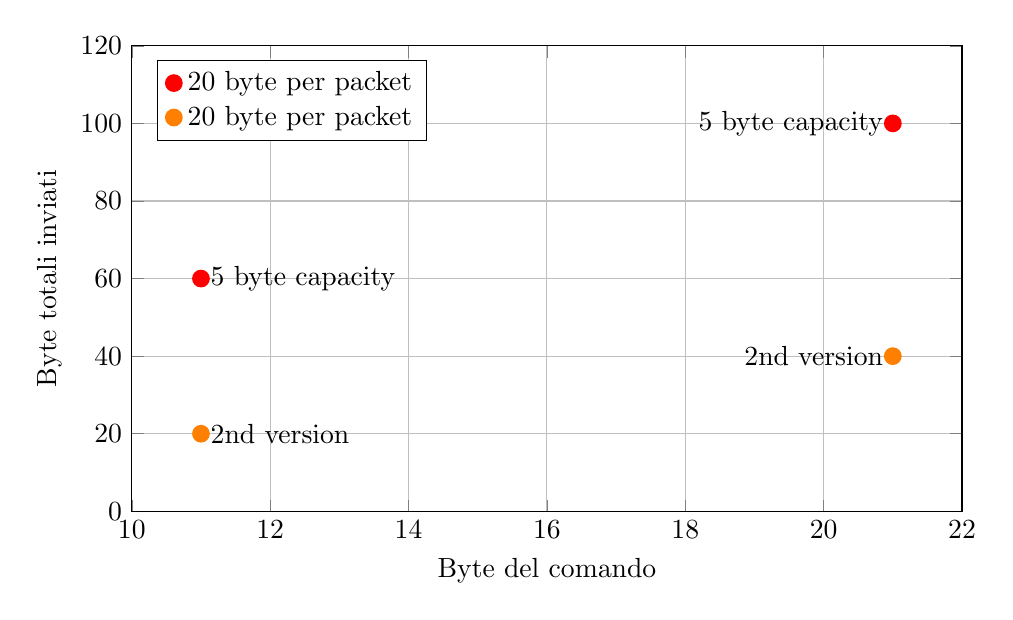
\begin{tikzpicture} 
    \tikzset{
    cmd11/.style={circle,fill=red,inner sep=2pt},
    cmd21/.style={circle,fill=blue,inner sep=2pt}
}
\begin{axis}[
    xlabel={Byte del comando}, 
    ylabel={Byte totali inviati},
    grid=major,
    width=\textwidth,
    height=0.618\textwidth, 
    domain=10:22,
    ymin=0,
    ymax=120, 
    legend pos=north west,
    legend entries={20 byte per packet, 20 byte per packet}
]  
% Plot points
\addplot[only marks, mark=*, mark size=3pt, red] 
coordinates {(11,60) (21,100)}; 
\addplot[only marks, mark=*, mark size=3pt, orange] 
coordinates {(11,20) (21,40)}; 
% Add labels for the points 
\node[right] at (axis cs:11,60) {5 byte capacity}; 
\node[left] at (axis cs:21,100) {5 byte capacity}; 

\node[right] at (axis cs:11,20) {2nd version}; 
\node[left] at (axis cs:21,40) {2nd version}; 

\end{axis}
\end{tikzpicture}
\caption{Analisi tempi esecuzione \textit{Timestamp}} 
\label{table:timestamp:bytetotali:bytecomando}
\end{center}  
Dall'analisi segue che il metodo \hyperref[echo:casoA]{A} non riuslta il migliore. 
Infatti analizzando il caso in cui si usasse anche l'intera dimesnione dei campi \textit{timestamp} [Tabella:\ref{table:timestamp:bytetotali:bytecomando} Arancione]; 
si avrà una notevole differenza di bytes spediti totalmente rispetto alla controparte
\footnote{Questo perchè porta la capacitò del pacchetto a \textit{5 bytes} a \textbf{14 bytes}}. 
Tuttavia l'uso di questi campi risulta non possibile siccome le ore, i minuti e i secondi hanno un range di valori accettati e no
\footnote{I secondi, come i minuti devono essere compresi fra 0 e 59 mentre le ore fra 0 e 23}. 
Questo porta all'impossibilità di inserimento di alcune informazioni. 
In particoalre limita la possibilità di usare i caratteri il cui codice ASCII non è compreso nel range.   
\vspace{1ex} \newline
Una modifica per risolvere la cosa è l'inserimento diretto diretto nel campo. 
Tuttavia questo porterà a valori di tempo scostanti: 
\begin{lstlisting}[
    language=Python, basicstyle=\tiny, firstnumber=0, numbers=left, numberstyle=\tiny, xleftmargin=5mm
    %
    ,emph={data}, emphstyle=\color{red} 
    ,emph={[2]index},emphstyle={[2]\color{blue}} 
    ,emph={[3]}, emphstyle={[3]\color{olive}} 
    ,literate={.}{{\char46}}1 {:}{{\char58}}1 
] 
data="echo 'Ciao'".encode() 
for index in range(0, len(data), 12): 
    print(f"Byte data: {int.from_bytes(data[index:index+4])}")
    print(f"Byte data: {int.from_bytes(data[index+5:index+8])}") 
    print(f"Byte data: {int.from_bytes(data[index+8:index+12])}") 
\end{lstlisting} 
\label{code:timestamp:casoB}
\captionof{lstlisting}{Si usa l'intero Timestamp per i dati}
\begin{lstlisting} [
    language=Python, basicstyle=\tiny, firstnumber=0, numbers=left, numberstyle=\tiny, xleftmargin=5mm
    %
    ,emph={data, icmp_ts_ori, icmp_ts_rx, icmp_ts_tx}, emphstyle=\color{red} 
    ,emph={[2]index, data_pkt},emphstyle={[2]\color{blue}} 
    ,emph={[3]current_time, midnight}, emphstyle={[3]\color{olive}} 
    ,literate={.}{{\char46}}1 {:}{{\char58}}1 
] 
#Output 
Byte data: 1701013615
Byte data: 2573161
Byte data: 6385447
\end{lstlisting} 
\label{code:timestamp:casoB:output}
\captionof{lstlisting}{Output del codice} 
\vspace{1ex} 
Ciò risulta sconveniente siccome, per come si sono definiti i campi di timestamp, questi tempi dovrebbero essere l'uno il successivo dell'altro. 
\vspace{2ex} \newline 
Questo limite non è presente nel campo \textit{milliseocndi} siccome il suo intervallo arriva sino a \href{https://docs.python.org/3.11/library/datetime.html#datetime.datetime.microsecond}{1000}. 
Inserendo un singolo byte il massimo valore inseribile è $2^8-1=255$. 
Il che copre tutti i possibili caratteri possibili, siccome in ASCII ognuno di essi è un singolo byte. 
\vspace{1ex} \newline 
Si procede quindi sulla strada del caso \hyperref[timestamp:casoA]{A} ricavando dal byte da inserire, l'intero risultante e poi lo si moltiplica per $10^3$.
Quest'ultimo valore sarà quello che si inserirà nel campo \textit{millisecondi}. 
Dopodichè una volta definito il timestamp, si noterà che in esso gli ultimi tre deciamli finali contengono il carattere inserito (\href{https://www.ascii-code.com/it}{espresso in decimale}). 
\vspace{1ex} \newline
\begin{lstlisting}[
    language=Python, basicstyle=\tiny, firstnumber=0, numbers=left, numberstyle=\tiny, xleftmargin=5mm
    %
    ,emph={data, icmp_ts_ori, icmp_ts_rx, icmp_ts_tx}, emphstyle=\color{red} 
    ,emph={[2]index, data_pkt},emphstyle={[2]\color{blue}} 
    ,emph={[3]current_time, midnight}, emphstyle={[3]\color{olive}} 
    ,literate={.}{{\char46}}1 {:}{{\char58}}1 
] 
data="echo 'Ciao'".encode() 
for index in range(0, len(data), 12): 
    icmp_id=icmp_id=(data[index]<<8)+data[index+1] 

    current_time=datetime.datetime.now(datetime.timezone.utc) 
    midnight = current_time.replace(
        hour=0, minute=0, second=0, microsecond=0
    ) 

    data_pkt=int.from_bytes(data[index+2:index+3]) *10**3
    current_time=current_time.replace(microsecond=data_pkt)
    icmp_ts_ori=int((current_time - midnight).total_seconds() * 1000) 
    print(f"Byte data: {data[index+2:index+3]}")
    print(f"Data pkt: {data_pkt}")
    print(f"Timestamp: {icmp_ts_ori}") 
    
    data_pkt=int.from_bytes(data[index+3:index+4]) *10**3 
    if current_time.second+1<60:
        current_time=current_time.replace(
            second=current_time.second+1, microsecond=data_pkt
        ) 
    else:
        current_time=current_time.replace(
            minute=current_time.minute+1
            ,second=(current_time.second+1)%60
            , microsecond=data_pkt
        ) 
    icmp_ts_rx=int((current_time - midnight).total_seconds() * 1000) 
    print(f"Byte data: {data[index+3:index+4]}")
    print(f"Data pkt: {data_pkt}")
    print(f"Timestamp: {icmp_ts_rx}") 

    data_pkt=int.from_bytes(data[index+4:index+5]) *10**3 
    if current_time.second+1<60: 
        current_time=current_time.replace(
            second=current_time.second+1, microsecond=data_pkt
        )
    else: 
        current_time=current_time.replace(
            minute=current_time.minute+1
            ,second=(current_time.second+1)%60
            ,microsecond=data_pkt
        )
    icmp_ts_tx=int((current_time - midnight).total_seconds() * 1000) 
    print(f"Byte data: {data[index+4:index+5]}")
    print(f"Data pkt: {data_pkt}")
    print(f"Timestamp: {icmp_ts_tx}")
\end{lstlisting} 
\label{code:timestamp:casoA}
\captionof{lstlisting}{Si usa un byte del Timestamp per i dati}
\begin{lstlisting} [
    language=Python, basicstyle=\tiny, firstnumber=0, numbers=left, numberstyle=\tiny, xleftmargin=5mm
    %
    ,emph={data, icmp_ts_ori, icmp_ts_rx, icmp_ts_tx}, emphstyle=\color{red} 
    ,emph={[2]index, data_pkt},emphstyle={[2]\color{blue}} 
    ,emph={[3]current_time, midnight}, emphstyle={[3]\color{olive}} 
    ,literate={.}{{\char46}}1 {:}{{\char58}}1 
] 
#Output 
ICMP id: 25955
Byte data: b'h'
    Data pkt: 104000
    Timestamp ori: 38494104
Byte data: b'o'
    Data pkt: 111000
    Timestamp rx: 38495111
Byte data: b' '
    Data pkt: 32000
    Timestamp tx: 38496032
ICMP id: 10051
Byte data: b'i'
    Data pkt: 105000
    Timestamp ori: 38494105
Byte data: b'a'
    Data pkt: 97000
    Timestamp rx: 38495097
Byte data: b'o'
    Data pkt: 111000
    Timestamp tx: 38496111
ICMP id: 9984
\end{lstlisting} 
\label{code:timestamp:casoA:output}
\captionof{lstlisting}{Output del codice}



\subsubsection{Information Request or Information Reply Message (ICMPv4)} 
Nel protocollo \textbf{ICMPv4} la tipologia di messaggio \textit{Information}, viene usata per consentire a un host di scoprire il numero della rete in cui si trova. 
E quindi per capire se si trova nella stesse rete dell'host che risponde. 
L'identificatore e il numero di sequenza possono essere utilizzati dal mittente del pacchetto per facilitare l'abbinamento delle risposte con le richieste.
\vspace{1ex} \newline 
Questo messaggio può essere inviato con la rete sorgente nel campo mittente e 
la destinazione nell'intstazione IP pari a zero (ciò significa "questa" rete). 
Tuttavia l'intestazione IP presente nel messaggio di risposta dovrà essere inviata con gli indirizzi IP completamente specificati.
\vspace{2ex} \newline 
Per creare un messaggio di risposta, gli indirizzi di origine e di destinazione vengono invertiti,
il codice da 15 viene modificato in 16 e il checksum viene ricalcolato. 

\subsubsection*{Struttura del pacchetto} 
\begin{bytefield}[bitwidth=1.1em]{32} 
    %\bitbox{8}{0} & \bitbox{8}{1} & \bitbox{8}{2} & \bitbox{8}{3} \\
    \bitheader{0-31} \\
    \bitbox{8}{Type (1B)} & \bitbox{8}{Code (1B)} & \bitbox{16}{Checksum (2B)} \\
    \bitbox{16}{Identifier (2B)} && \bitbox{16}{Sequence Number (2B)} 
\end{bytefield}
I campi sono i seguenti: 
\begin{itemize}
    \item Type: 15 per i messaggi Information Request; 16 per i messaggi Information Reply. 
    \item Code: 0 che può essere ricevuto sia da un gateway che da un host
    \item Checksum: è il complemento a 16 bit del complemento a uno relativo alla somma del messaggio ICMP 
    (che inizia con il campo Type). Verrà calcolato se il campo è zero. 
    \item Identifier: se il codice = 0; l'identificatore serve per facilitare la corrispondenza tra le richieste Echo e le Risposte Echo. Può essere zero. 
    \item Sequence Number: se il codice = 0; il numero di sequenza serve per facilitare la corrispondenza tra le richieste Echo e le Risposte Echo. Può essere zero. 
\end{itemize}
\vspace{1ex} 
Si sfrutteranno quindi i campi nel seguente modo: 
\begin{itemize}
    \item Il campo \textbf{checksum} non è utilizzabile. 
    Essendo il complemento ad 1 del contenuto del pacchetto, se non combaciasse il pacchetto verrebbe scartato. 
    \item Il campo \textbf{identifier} che siccome serve a definire un identificativo delle richieste, può essere un qualsiasi valore. 
    \item Il campo di \textbf{sequenza} potrebbe essere utilizzato per inserire le informazioni; 
    tuttavia, dalle specifiche \href{https://www.rfc-editor.org/rfc/rfc792.html#:~:text=Information%20Request%20or%20Information%20Reply%20Message}{RFC 792}, esso viene incrementato ad ogni richiesta inviata. %20
    Quindi se il valore del campo sarà troppo variabile, potrebbe risultare sospetto. 
\end{itemize} 

\subsubsection*{Analisi complessiva} 
Per l'analisi supponiamo di mandare due comandi che sono: 
\begin{itemize}
    \item \textbf{echo 'Ciao'}: che sono \textit{11 byte} (e quindi \textit{88 bit}\footnote{\label{note:information:analisi}Ciò sarà utile per i \textit{Timing Covert Channel}})
    \item \textbf{cd /home/marco; ls -l}: che sono \textit{21 byte}  (e quindi \textit{168 bit}\textsuperscript{\ref{note:information:analisi}}) %\footnotemark[2]
\end{itemize}
Sappiamo che nel caso migliore la capacità di trasmissione di ogni pacchetto è \textbf{2 byte} \label{information:casoA}; 
questo perchè il campo \textit{identifier} ha una lunghezza di soli \textit{2 byte}. %20 
\begin{itemize}
    \item Ogni pacchetto del caso (che chiameremo \hyperref[information:casoA]{A}) trasporterà \textbf{8 byte}
    \footnote{8 per i campi ICMP} 
\end{itemize} 
Ora si analizza quanti pacchetti saranno necessari per inviare i comandi. \newline
Nel caso si mandasse il comando \textbf{information 'Ciao'} il numero di pacchetti necessari sarebbere: 
\begin{itemize}
    \item Caso \hyperref[information:casoA]{A}: Sarebbero necessari \textit{6 pacchetti}. 
    E quindi siccome ogni pacchetto trasporta \textit{8 byte}; si spediranno in totale \textbf{48 byte}. 
\end{itemize} 
Ora analiziamo il comando \textbf{cd /home/marco; ls -l} e quanti pacchetti saranno necessari: 
\begin{itemize}
    \item Caso \hyperref[information:casoA]{A}: siccome è di \textit{21 byte}, servirebbero \textit{11 pacchetti}. 
    Quindi siccome ogni pacchetto trasporta \textit{8 byte}; si spediranno in totale \textbf{88 byte}. 
\end{itemize}

\begin{center} 
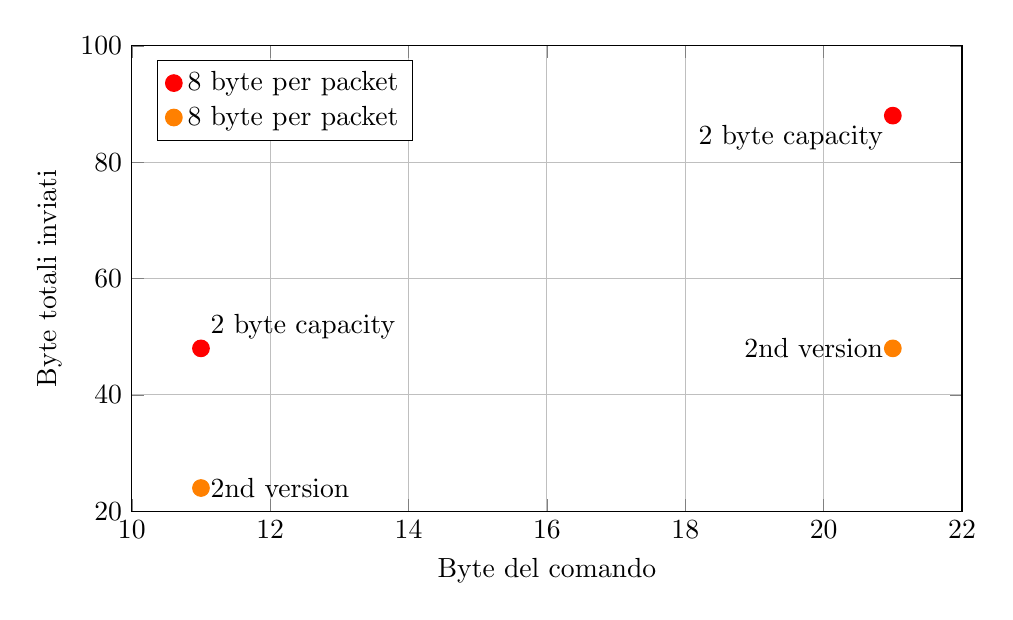
\begin{tikzpicture} 
    \tikzset{
    cmd11/.style={circle,fill=red,inner sep=2pt},
    cmd21/.style={circle,fill=blue,inner sep=2pt}
}
\begin{axis}[
    xlabel={Byte del comando}, 
    ylabel={Byte totali inviati},
    grid=major,
    width=\textwidth,
    height=0.618\textwidth, 
    domain=10:22,
    ymin=20,
    ymax=100, 
    legend pos=north west,
    legend entries={8 byte per packet, 8 byte per packet}
]  
% Plot points
\addplot[only marks, mark=*, mark size=3pt, red] 
coordinates {(11,48) (21,88)}; 
\addplot[only marks, mark=*, mark size=3pt, orange] 
coordinates {(11,24) (21,48)}; 
% Add labels for the points 
\node[above right] at (axis cs:11,48) {2 byte capacity}; 
\node[below left] at (axis cs:21,88) {2 byte capacity}; 

\node[right] at (axis cs:11,24) {2nd version}; 
\node[left] at (axis cs:21,48) {2nd version}; 

\end{axis}
\end{tikzpicture}
\caption{Analisi tempi esecuzione \textit{Information}} 
\label{table:information:bytetotali:bytecomando}
\end{center}
Dall'analisi segue che il metodo \hyperref[information:casoA]{A} non riuslta il migliore. 
Infatti analizzando il caso in cui si usasse anche il campo di \textit{sequenza} [Tabella:\ref{table:information:bytetotali:bytecomando} Arancione]; 
si avrà una notevole differenza di bytes spediti totalmente rispetto al caso \hyperref[information:casoA]{A}. 
\vspace{1ex} \newline
Tuttavia siccome l'uso di questo campo comporta una maggiore visibilità, 
si sceglie di non usarlo e correre il rischio. 
Questo comporterà l'invio di un maggior numero di bytes; 
che anche ciò potrebbe rivelare il Covert Channel. 
\vspace{1ex} \newline 
Si è scelto quindi di usare il metodo \hyperref[information:casoA]{A} ed affidarsi ai meccanismi di difesa presenti nella vittima; 
nella speranza che un numero elevato di pacchetti possano essere considerati innocqui.




